% !TEX program = lualatex
\documentclass[a4paper,12pt]{article}

% Layout and fonts
\usepackage[top=2.5cm,bottom=2.5cm,left=2.5cm,right=2.5cm]{geometry}
\usepackage{fontspec}

% Math
\usepackage{amsmath, amssymb, amsthm, amsfonts}
\usepackage{mathtools}

% Hyperreferences
\usepackage{xcolor}
\usepackage[
    colorlinks=true,
    urlcolor=red,
    linkcolor=blue,
    citecolor=teal
]{hyperref}
\usepackage{xurl} % nicer URL line breaks
\urlstyle{same} % URLs formatting same as text

% Text formatting
\usepackage{ragged2e} % different text alignments
\usepackage{csquotes} % quotations

% Figures
\usepackage{graphicx}
\usepackage[section,below]{placeins}
\usepackage{flafter}
\usepackage{caption} % customize captions
\captionsetup{labelfont=bf, font=small}
\renewcommand{\topfraction}{0.85}
\renewcommand{\bottomfraction}{0.7}
\renewcommand{\textfraction}{0.1}
\renewcommand{\floatpagefraction}{0.8}

% Tables
\usepackage{booktabs} % extra commands for tabular env.
\makeatletter
\def\fps@table{!htbp}
\makeatother

% Tables produced by modelsummary (tinytable / tabularray)
\usepackage{tabularray}
\usepackage{codehigh}
\usepackage[normalem]{ulem}
\usepackage{siunitx}
\UseTblrLibrary{booktabs}
\UseTblrLibrary{siunitx}
\newcommand{\tinytableTabularrayUnderline}[1]{\underline{#1}}
\newcommand{\tinytableTabularrayStrikeout}[1]{\sout{#1}}
\NewTableCommand{\tinytableDefineColor}[3]{\definecolor{#1}{#2}{#3}}
\SetTblrStyle{caption-tag}{font=\small\bfseries} % table captions like figure captions
\SetTblrStyle{caption-sep}{font=\small\bfseries}
\SetTblrStyle{caption-text}{font=\small}

% Bibliography
\usepackage{natbib}
\bibliographystyle{ecta}
\usepackage[nottoc, notlot, notlof]{tocbibind} % References in the table of contents
\settocbibname{References} % title of the bibliography

% Title
\title{Life Expectancy, Income and Geography:\\ An Empirical Analysis of the Gapminder Data}
\author{Nikita Zhdanov\\[0.3em]
    \small Scientific Working with R and \LaTeX{}\\
    \small Vienna University of Economics and Business}
\date{\today}

\begin{document}

\maketitle

\begin{abstract}
    \noindent This report studies the cross-country determinants of life expectancy with the \texttt{gapminder} dataset. In 1997, income per person and the continent of a country together explain 82\% of the variation in life expectancy: a 1\% higher GDP per capita is associated with about 0.056 additional years, and African countries live 8--9 years shorter than other countries with the same income. Total GDP is a much weaker predictor, both in sample and when predicting the 2002 values. Finally, Austria's life expectancy grows so steadily over 1952--2007 that a simple random walk with drift forecasts its 2007 value within 0.4 years.
\end{abstract}

\newpage

\tableofcontents

\listoffigures

\listoftables

\newpage

% =====================================================================
\section{Description of the data}
\label{sec:data}

The analysis uses the \texttt{gapminder} dataset from the R package of the same name \citep{bryan2025gapminder}, an excerpt of the data collected by the \href{https://www.gapminder.org/}{Gapminder Foundation}. It covers 142 countries in five-year steps from 1952 to 2007 and contains life expectancy at birth (\texttt{lifeExp}, in years), population (\texttt{pop}) and GDP per capita (\texttt{gdpPercap}, in inflation-adjusted US dollars). The target variable is life expectancy. I add total GDP, defined as
\begin{equation}
    \texttt{gdp} = \texttt{gdpPercap} \times \texttt{pop} \, ,
    \label{eq:gdp}
\end{equation}
and create two cross-sections: \texttt{df} with all countries in 1997 and \texttt{df2} with all countries in 2002. Sections \ref{sec:data} and \ref{sec:regression} use only the 1997 data; the 2002 data serve as a test set in Section~\ref{sec:prediction}. All computations were done in R \citep{rcore2025}, and the tables were produced with \texttt{modelsummary} \citep{arelbundock2022modelsummary}.

\subsection{Summary statistics}

Table~\ref{tab:summary} reports summary statistics for the four numeric variables.\footnote{
    The column \texttt{year} is numeric as well, but it is constant (1997) in this subsample. It therefore carries no information and has no defined correlation with the other variables.
}

\begin{table}
\centering
\begin{talltblr}[         %% tabularray outer open
caption={Summary statistics, 1997 (142 countries) \label{tab:summary}},
]                     %% tabularray outer close
{                     %% tabularray inner open
colspec={Q[]Q[]Q[]Q[]Q[]Q[]Q[]},
hline{2}={1-7}{solid, black, 0.05em},
hline{1}={1-7}{solid, black, 0.08em},
hline{6}={1-7}{solid, black, 0.08em},
column{1}={}{halign=l},
column{2-7}={}{halign=r},
}                     %% tabularray inner close
& N & Mean & SD & Min & Median & Max \\
Life expectancy (years) & 142 & \num{65.0} & \num{11.6} & \num{36.1} & \num{69.4} & \num{80.7} \\
GDP per capita (USD) & 142 & \num{9090.2} & \num{10171.5} & \num{312.2} & \num{4781.8} & \num{41283.2} \\
Population (millions) & 142 & \num{38.8} & \num{133.4} & \num{0.1} & \num{9.7} & \num{1230.1} \\
GDP (billion USD) & 142 & \num{288.8} & \num{946.5} & \num{0.2} & \num{37.5} & \num{9761.4} \\
\end{talltblr}
\end{table}


\paragraph{Life expectancy.} The average country has a life expectancy of 65.0 years, but the median is higher (69.4 years), so the distribution is \emph{skewed to the left}: large share of countries is clustered above 70 years (65 of 142), while a long tail of low values (21 countries below 50 years) pulls the mean down. The spread is large, with a standard deviation of 11.6 years and a range of 44.6 years, from Rwanda (36.1) to Japan (80.7).

\paragraph{Income and size.} The other three variables are strongly \emph{skewed to the right}. Mean GDP per capita (\$9{,}090) is almost twice the median (\$4{,}782), and it ranges from \$312 (Congo, Dem.\ Rep.) to \$41{,}283 (Norway), a factor of about 130. Population and total GDP are dominated by a few very large countries: China and India have 1{,}230 and 959 million inhabitants, against a median of 9.7 million, and the United States alone produces a GDP of \$9{,}761 billion, against a median of \$37.5 billion. This skewness is the reason why the variables enter the graphs and regressions below in logarithms.

\FloatBarrier
\subsection{Correlations}

Table~\ref{tab:correlations} reports the pairwise Pearson correlations. Life expectancy is strongly positively correlated with GDP per capita (0.70), only weakly with total GDP (0.25), and essentially uncorrelated with population (0.05). Total GDP is correlated with both population (0.43) and GDP per capita (0.37), since by \eqref{eq:gdp} it is their product, while population and GDP per capita are unrelated ($-0.05$). Because the variables are so skewed, the correlations are even stronger on the log scale: life expectancy has a correlation of 0.86 with log GDP per capita and 0.62 with log GDP.

\begin{table}
\centering
\begin{talltblr}[         %% tabularray outer open
caption={Pairwise Pearson correlations, 1997 (142 countries) \label{tab:correlations}},
]                     %% tabularray outer close
{                     %% tabularray inner open
colspec={Q[]Q[]Q[]Q[]Q[]},
hline{2}={1-5}{solid, black, 0.05em},
hline{1}={1-5}{solid, black, 0.08em},
hline{6}={1-5}{solid, black, 0.08em},
column{1}={}{halign=l},
column{2-5}={}{halign=r},
}                     %% tabularray inner close
& Life expectancy & GDP per capita & Population & GDP \\
Life expectancy & 1 & . & . & . \\
GDP per capita & \num{.70} & 1 & . & . \\
Population & \num{.05} & \num{-.05} & 1 & . \\
GDP & \num{.25} & \num{.37} & \num{.43} & 1 \\
\end{talltblr}
\end{table}


\FloatBarrier
\subsection{Visualisations}

\paragraph{Income.} Figure~\ref{fig:scatter} shows a strong, roughly linear relation between log GDP per capita and life expectancy: richer countries can afford better healthcare, nutrition and sanitation. Since the relation is linear in logs, each 1\% increase in income adds about the same number of years, so in absolute dollars the gains diminish: an extra \$1{,}000 matters far more in a poor country than in a rich one. The countries furthest below the line are in Southern Africa (Angola, Botswana, Zambia), a region hit hard by HIV/AIDS.

\begin{figure}[!htbp]
    \centering
    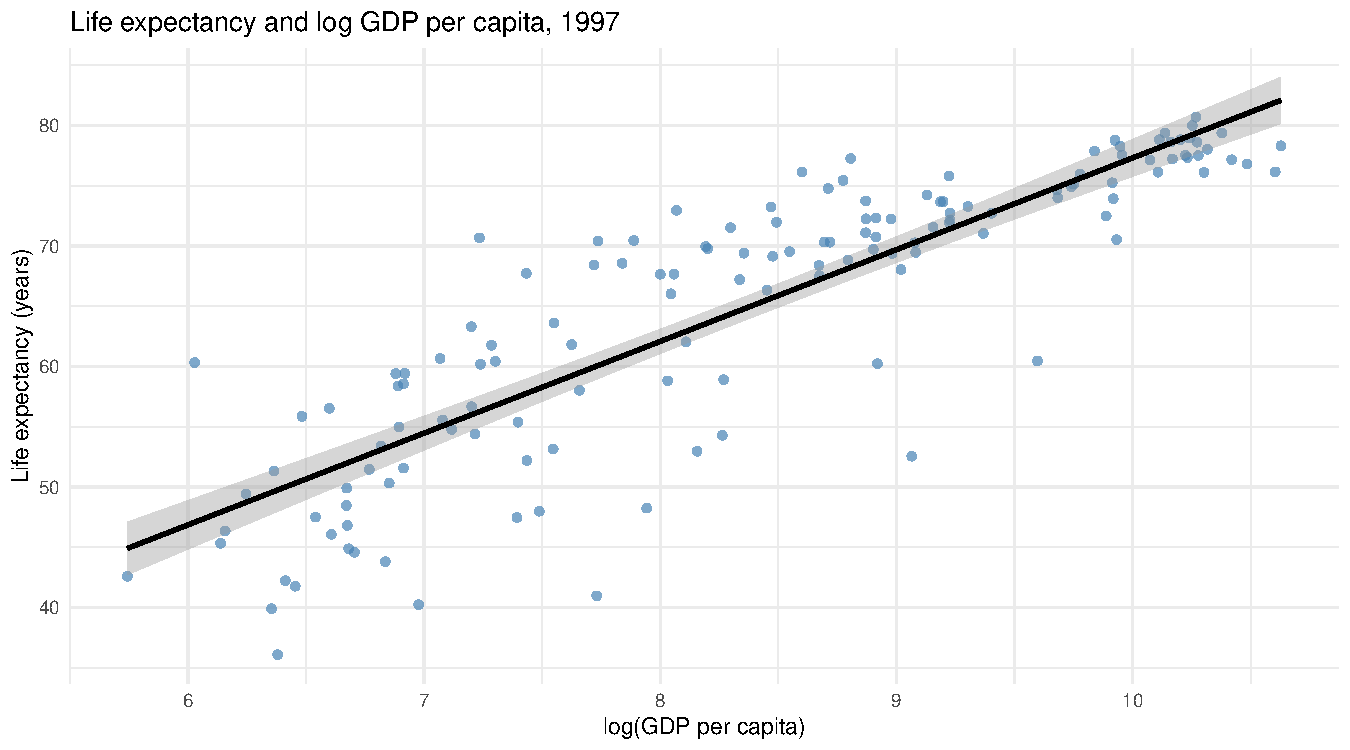
\includegraphics[width=0.9\textwidth]{figures/lifeExp_and_logGDPperCapita.pdf}
    \caption[Life expectancy and log GDP per capita]{Life expectancy and log GDP per capita, 1997. The black line is an OLS fit with its 95\% confidence band.}
    \label{fig:scatter}
\end{figure}

\paragraph{Continents.} Figure~\ref{fig:boxplot} shows that Africa has by far the lowest median life expectancy (52.8 years) and the widest spread in the middle of the distribution (interquartile range 11.9 years), consistent with Figure~\ref{fig:scatter}, since most low-income countries are African. Asia, the Americas and Europe have medians between 70 and 76 years. Asia is the most dispersed of the three, from Japan (80.7, the highest value in the data) to Afghanistan (41.8), Yemen and Iraq, while the low outliers of the Americas are Haiti (56.7) and Bolivia (62.0). Europe is the most compact continent (standard deviation 3.1 years), and its 25th percentile (73.0) lies above both the Americas' median (72.1) and Asia's 75th percentile (72.5).\footnote{
    Oceania consists of only two countries, Australia and New Zealand, and its box should be read with caution.
}

\begin{figure}[!htbp]
    \centering
    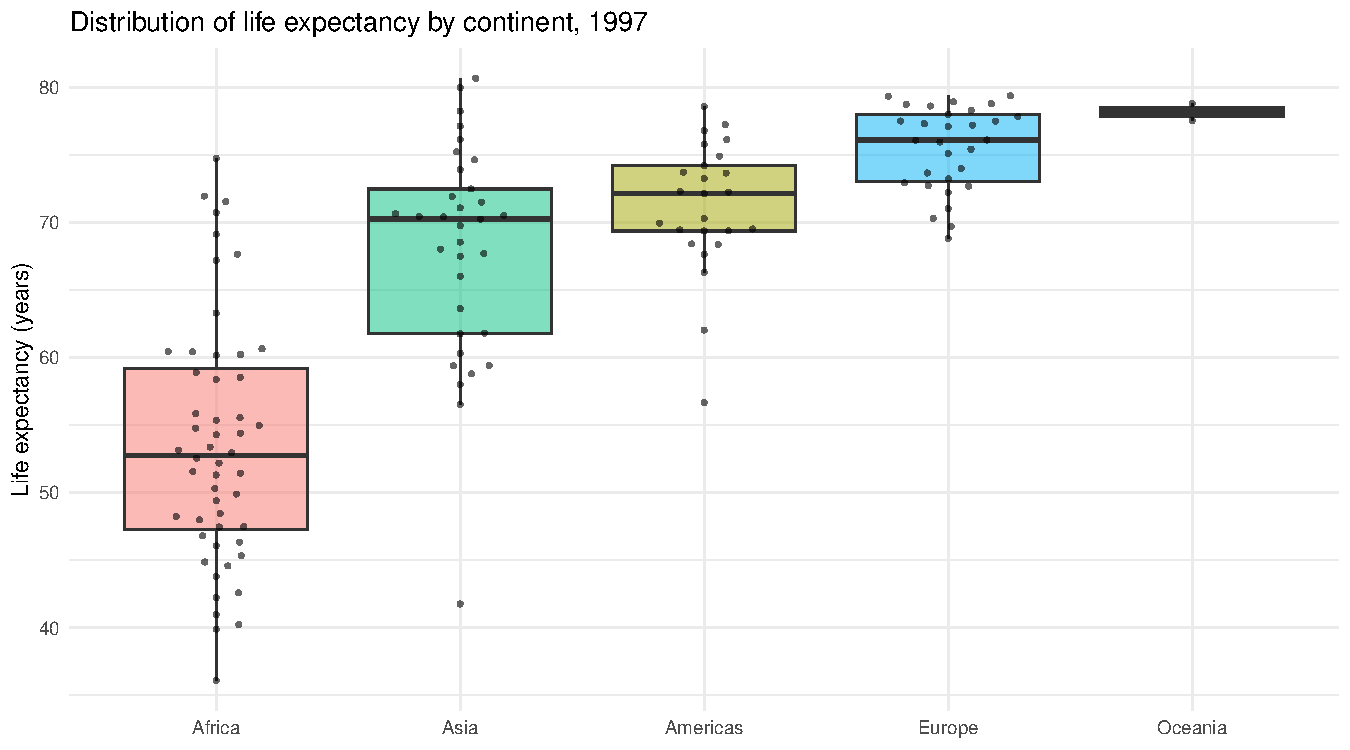
\includegraphics[width=0.9\textwidth]{figures/distr_lifeExp_by_continent.pdf}
    \caption[Life expectancy by continent]{Distribution of life expectancy by continent, 1997. Each point is a country; continents are ordered by their median.}
    \label{fig:boxplot}
\end{figure}

\paragraph{Income within continents.} Figure~\ref{fig:scatter-continent} combines both determinants. The income gradient is positive within every continent, so income matters regardless of the region. At the same income level, however, African countries lie well below the others: the African line is 7--9 years lower at low and middle incomes, and the gap narrows as income rises. Continent therefore carries information beyond income, for example about the burden of disease. The slopes are fairly similar across continents, which supports a regression with one common income slope and continent dummies (Section~\ref{sec:regression}). The point sizes show that population does not line up with life expectancy: China and India lie where their income predicts.

\begin{figure}[!htbp]
    \centering
    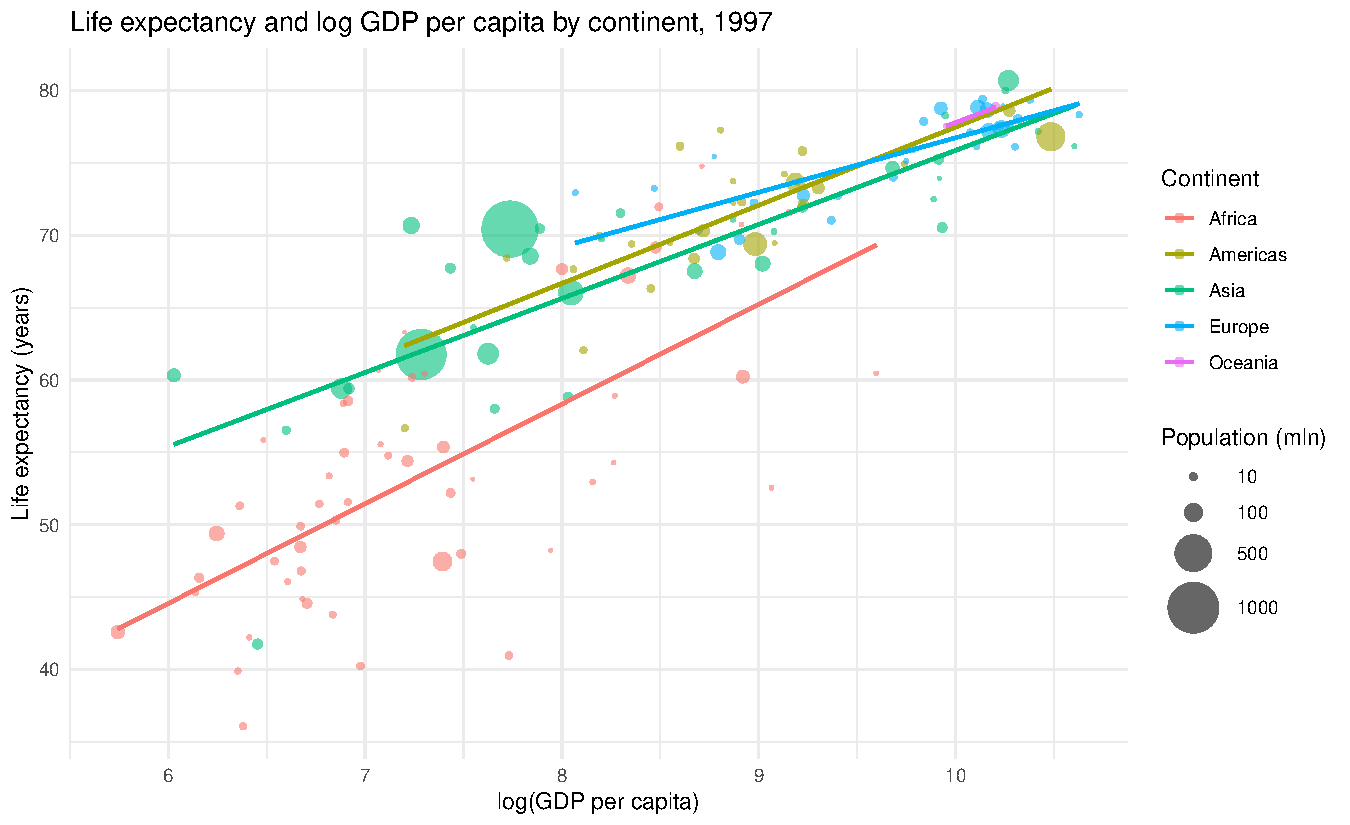
\includegraphics[width=0.9\textwidth]{figures/lifeExp_and_logGDPperCapita_by_continent.pdf}
    \caption[Life expectancy and log GDP per capita by continent]{Life expectancy and log GDP per capita by continent, 1997, with a separate OLS line for each continent. Point size is proportional to population.}
    \label{fig:scatter-continent}
\end{figure}

\paragraph{Total GDP and population.} Figure~\ref{fig:gdp-pop} replaces GDP per capita by total GDP and by population. Panel~A shows a moderate positive relation between log GDP and life expectancy, but with much more scatter than in Figure~\ref{fig:scatter} ($R^2$ of 0.38 against 0.75). In Panel~B the line for log population is almost flat (slope 0.48, $p = 0.45$), so country size is not related to life expectancy. Total GDP mixes income with country size, and only the income part matters; log GDP should therefore be the weaker predictor in Section~\ref{sec:regression}.

\begin{figure}[!htbp]
    \centering
    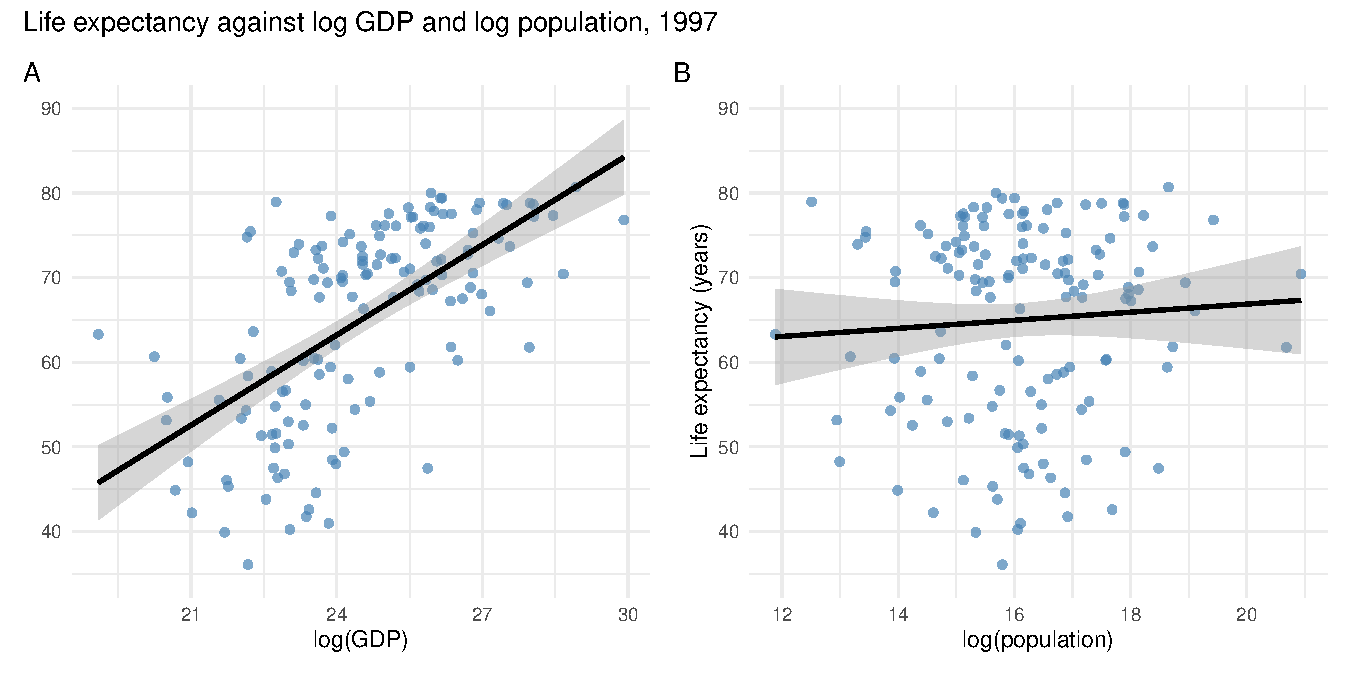
\includegraphics[width=\textwidth]{figures/lifeExp_and_logPop_logGDP.pdf}
    \caption[Life expectancy against log GDP and log population]{Life expectancy against log GDP (A) and log population (B), 1997, with OLS fits and 95\% confidence bands.}
    \label{fig:gdp-pop}
\end{figure}

% =====================================================================
\section{Linear regression}
\label{sec:regression}

I estimate two linear regressions by ordinary least squares (OLS) on the 1997 data:
\begin{align}
    \texttt{lifeExp}_i &= \beta_0 + \beta_1 \log(\texttt{gdpPercap}_i) + \sum_{c} \gamma_c \, D_{c,i} + \varepsilon_i \, , \label{eq:model1} \\
    \texttt{lifeExp}_i &= \beta_0 + \beta_1 \log(\texttt{gdp}_i) + \sum_{c} \gamma_c \, D_{c,i} + \varepsilon_i \, , \label{eq:model2}
\end{align}
where $D_{c,i}$ are dummy variables for the Americas, Asia, Europe and Oceania. Since every country belongs to exactly one continent, one dummy has to be left out; \textbf{Africa is the reference category}.\footnote{
    R uses the first level of a factor as the reference category, which for \texttt{continent} is Africa in alphabetical order. Choosing another reference would change the continent coefficients but not the fit of the model.
}
Each continent coefficient $\gamma_c$ is therefore the difference in life expectancy relative to an African country with the same income. Because income enters in logs, $\beta_1/100$ is the change in life expectancy (in years) associated with a 1\% increase in income, since $\log(1.01\,x) - \log(x) \approx 0.01$.

\subsection{Model 1: log GDP per capita}

Table~\ref{tab:model1} reports the estimates of model \eqref{eq:model1}. All coefficients are statistically significant: log GDP per capita and the dummies for the Americas, Asia and Europe at the 0.1\% level, and Oceania at the 5\% level ($p = 0.018$), whose estimate is imprecise because it rests on only two countries.

\begin{table}
\centering
\begin{talltblr}[         %% tabularray outer open
caption={OLS regression of life expectancy on log GDP per capita and continent, 1997 \label{tab:model1}},
note{}={+ p \num{< 0.1}, * p \num{< 0.05}, ** p \num{< 0.01}, *** p \num{< 0.001}},
note{ }={Reference continent: Africa. Standard errors in parentheses.},
]                     %% tabularray outer close
{                     %% tabularray inner open
width={0.7\linewidth},
colspec={X[]X[]},
hline{2}={1-2}{solid, black, 0.05em},
hline{14}={1-2}{solid, black, 0.05em},
hline{1}={1-2}{solid, black, 0.08em},
hline{17}={1-2}{solid, black, 0.08em},
column{2}={}{halign=c},
column{1}={}{halign=l},
}                     %% tabularray inner close
& Life expectancy \\
Constant & \num{12.629}*** \\
& (\num{3.353}) \\
log(GDP per capita) & \num{5.603}*** \\
& (\num{0.449}) \\
Americas & \num{9.050}*** \\
& (\num{1.386}) \\
Asia & \num{7.950}*** \\
& (\num{1.219}) \\
Europe & \num{8.669}*** \\
& (\num{1.555}) \\
Oceania & \num{9.083}* \\
& (\num{3.783}) \\
Observations & \num{142} \\
R² & \num{0.823} \\
Adjusted R² & \num{0.816} \\
\end{talltblr}
\end{table}


\begin{itemize}
    \item \textbf{Income.} The coefficient of 5.60 means that a 1\% increase in GDP per capita is associated with $5.60/100 \approx 0.056$ additional years of life expectancy, holding the continent fixed.
    \item \textbf{Continent.} Compared with an African country with the same GDP per capita, life expectancy is 9.1 years higher in the Americas, 8.0 years in Asia, 8.7 years in Europe and 9.1 years in Oceania. The non-African continents differ little from each other once income is controlled for: the raw gap between the European and African medians in Figure~\ref{fig:boxplot} (23 years) is mostly explained by income.
    \item \textbf{Constant.} The intercept (12.6) is the prediction for an African country with a GDP per capita of \$1, far outside the data, and has no meaningful interpretation.
    \item \textbf{Fit.} The model explains 82\% of the cross-country variation in life expectancy, compared with 75\% for log GDP per capita alone.
\end{itemize}

These results are associations in one cross-section and should not be read as causal effects.

\FloatBarrier
\subsection{Model 2: log GDP}

Table~\ref{tab:model2} reports model \eqref{eq:model2}, in which total GDP replaces GDP per capita. All coefficients are again significant: log GDP and the four continent dummies at the 0.1\% level, and the constant at the 1\% level.

\begin{table}
\centering
\begin{talltblr}[         %% tabularray outer open
caption={OLS regression of life expectancy on log GDP and continent, 1997 \label{tab:model2}},
note{}={+ p \num{< 0.1}, * p \num{< 0.05}, ** p \num{< 0.01}, *** p \num{< 0.001}},
note{ }={Reference continent: Africa. Standard errors in parentheses.},
]                     %% tabularray outer close
{                     %% tabularray inner open
width={0.7\linewidth},
colspec={X[]X[]},
hline{2}={1-2}{solid, black, 0.05em},
hline{14}={1-2}{solid, black, 0.05em},
hline{1}={1-2}{solid, black, 0.08em},
hline{17}={1-2}{solid, black, 0.08em},
column{2}={}{halign=c},
column{1}={}{halign=l},
}                     %% tabularray inner close
& Life expectancy \\
Constant & \num{22.530}** \\
& (\num{8.463}) \\
log(GDP) & \num{1.354}*** \\
& (\num{0.367}) \\
Americas & \num{14.666}*** \\
& (\num{1.857}) \\
Asia & \num{11.159}*** \\
& (\num{1.776}) \\
Europe & \num{18.134}*** \\
& (\num{1.888}) \\
Oceania & \num{20.438}*** \\
& (\num{5.114}) \\
Observations & \num{142} \\
R² & \num{0.654} \\
Adjusted R² & \num{0.641} \\
\end{talltblr}
\end{table}


\begin{itemize}
    \item \textbf{GDP.} A 1\% increase in total GDP is associated with only $1.35/100 \approx 0.014$ additional years of life expectancy, holding the continent fixed. This is roughly a quarter of the effect of GDP per capita. Since $\log(\texttt{gdp}) = \log(\texttt{gdpPercap}) + \log(\texttt{pop})$, total GDP mixes income, which matters, with country size, which does not (Figure~\ref{fig:gdp-pop}). A large GDP can belong to a rich country or simply to a big one, which dilutes the coefficient.
    \item \textbf{Continent.} The gaps relative to Africa are now much larger: 14.7 years for the Americas, 11.2 for Asia, 18.1 for Europe and 20.4 for Oceania. Because log GDP is a poor measure of living standards, the dummies absorb income differences that it fails to capture, for example the high income per person in Europe and Oceania.
    \item \textbf{Fit.} The $R^2$ falls from 0.82 to 0.65: replacing GDP per capita by total GDP clearly worsens the model.
\end{itemize}

% =====================================================================
\section{Prediction}
\label{sec:prediction}

To evaluate the models out of sample, both models of Section~\ref{sec:regression} are trained on the 1997 data (\texttt{df}) and used to predict life expectancy in 2002 (\texttt{df2}) from each country's 2002 values of income and continent. Accuracy is measured by the mean squared error,
\begin{equation}
    \text{MSE} = \frac{1}{n} \sum_{i=1}^{n} \left( \texttt{lifeExp}_{i,2002} - \widehat{\texttt{lifeExp}}_{i,2002} \right)^2 \, ,
    \label{eq:mse}
\end{equation}
and by its square root (RMSE), which is measured in years. The results are shown in Table~\ref{tab:mse}.

\begin{table}
\centering
\begin{talltblr}[         %% tabularray outer open
caption={Test MSE: models trained on 1997, evaluated on 2002 \label{tab:mse}},
]                     %% tabularray outer close
{                     %% tabularray inner open
colspec={Q[]Q[]Q[]},
hline{2}={1-3}{solid, black, 0.05em},
hline{1}={1-3}{solid, black, 0.08em},
hline{6}={1-3}{solid, black, 0.08em},
column{1}={}{halign=l},
column{2-3}={}{halign=r},
}                     %% tabularray inner close
Model & MSE & RMSE \\
(1) OLS: log(GDP per capita) + continent & \num{32.55} & \num{5.71} \\
(2) OLS: log(GDP) + continent & \num{50.78} & \num{7.13} \\
Decision tree & \num{34.85} & \num{5.90} \\
Random forest & \num{30.59} & \num{5.53} \\
\end{talltblr}
\end{table}


\paragraph{Comparison.} Model 1 with log GDP per capita predicts considerably better: its test MSE is 32.5 against 50.8 for model 2, about 36\% lower, and its typical error is 5.7 instead of 7.1 years. This agrees with the in-sample comparison of Section~\ref{sec:regression}: GDP per capita is the better predictor of life expectancy.

The largest errors come from Southern African countries such as Botswana and Swaziland, whose life expectancy fell between 1997 and 2002 because of the HIV/AIDS epidemic.

\subsection{Extension: tree-based models}
\label{sec:trees}

As a benchmark for model 1, I also train a decision tree \citep{therneau2025rpart} and a random forest of 500 trees \citep{liaw2002randomforest} on the same data and the same information, $\texttt{lifeExp} \sim \texttt{gdpPercap} + \texttt{continent}$.\footnote{
    Logarithms are not needed here, since a tree splits on thresholds and the ordering of the countries does not change under a log transformation.
}
Their test errors are included in Table~\ref{tab:mse}.

\begin{figure}[!htbp]
    \centering
    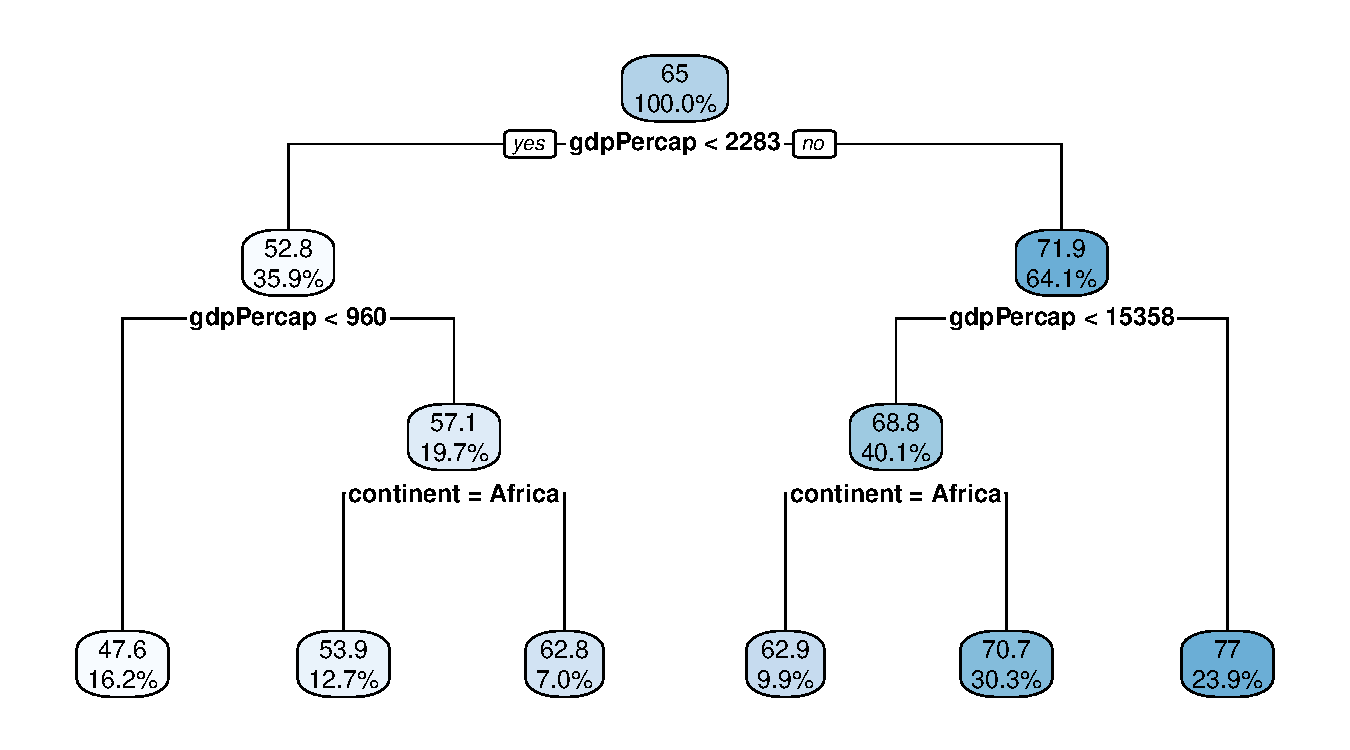
\includegraphics[width=0.9\textwidth]{figures/decision_tree.pdf}
    \caption[Decision tree for life expectancy]{Decision tree for life expectancy, trained on 1997. Each node shows the predicted life expectancy and the share of countries it contains.}
    \label{fig:tree}
\end{figure}

The single tree in Figure~\ref{fig:tree} is slightly worse than model 1 (MSE 34.9): it predicts only six distinct values, a coarse step function of income. Its first split is at a GDP per capita of about \$2{,}300, and \enquote{continent = Africa} appears in two later splits --- the same two determinants as in the regression. The random forest is the best model (MSE 30.6, about 6\% below model 1): averaging many trees smooths the steps and captures non-linearities and interactions, such as the different income slopes in Figure~\ref{fig:scatter-continent}, without specifying them. The gain is small, and its largest errors are the same countries as before. The better predictions come at a cost, however: unlike the regression, the forest has no coefficients that can be interpreted.

% =====================================================================
\section{Time series: Austria and the United States}
\label{sec:timeseries}

Figure~\ref{fig:ts} shows the full time series of life expectancy in Austria and the United States. Both series rise steadily over the whole period. The United States starts 1.6 years ahead (68.4 against 66.8 years in 1952) and stays ahead for four decades, but Austria improves faster: by 13.0 years over 1952--2007, against 9.8 years for the United States, whose growth slows noticeably after 1980. The gap shrinks to almost zero in 1987--1992, Austria overtakes the United States between 1992 and 1997, and in 2007 it is 1.6 years ahead (79.8 against 78.2) --- a full reversal of the 1952 position.

\begin{figure}[!htbp]
    \centering
    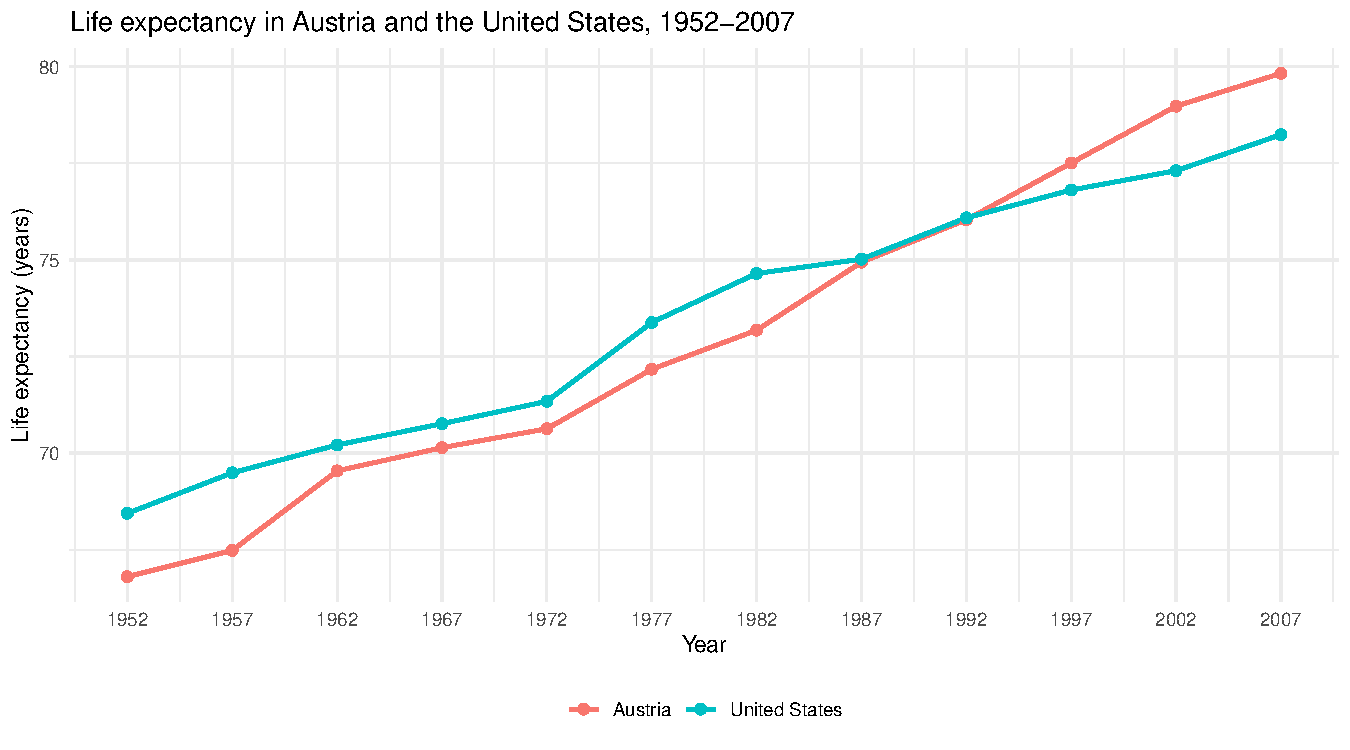
\includegraphics[width=0.9\textwidth]{figures/lifeExp_Austria_US.pdf}
    \caption[Life expectancy in Austria and the United States]{Life expectancy in Austria and the United States, 1952--2007.}
    \label{fig:ts}
\end{figure}

\subsection{Forecasting Austria's life expectancy in 2007}

The Austrian series has a steady upward trend and no seasonality, so a simple trend method is appropriate. I use a \textbf{random walk with drift}, estimated with the \texttt{fable} package \citep{oharawild2026fable} on the eleven observations from 1952 to 2002. Its forecast for 2007 is the last observed value plus the average five-year change over the training period:
\begin{equation}
    \widehat{y}_{2007} = y_{2002} + \frac{y_{2002} - y_{1952}}{10} = 78.98 + \frac{78.98 - 66.80}{10} \approx 80.20 \, .
    \label{eq:drift}
\end{equation}

The actual value in 2007 is 79.83, so the forecast is 0.37 years (0.5\%) too high, and the actual value lies well inside the 95\% prediction interval (Figure~\ref{fig:forecast}). The forecast slightly overshoots because the last increase (1997--2002) was unusually large. Because Austrian life expectancy grows so regularly, even this simple method forecasts it within less than half a year.

\begin{figure}[!htbp]
    \centering
    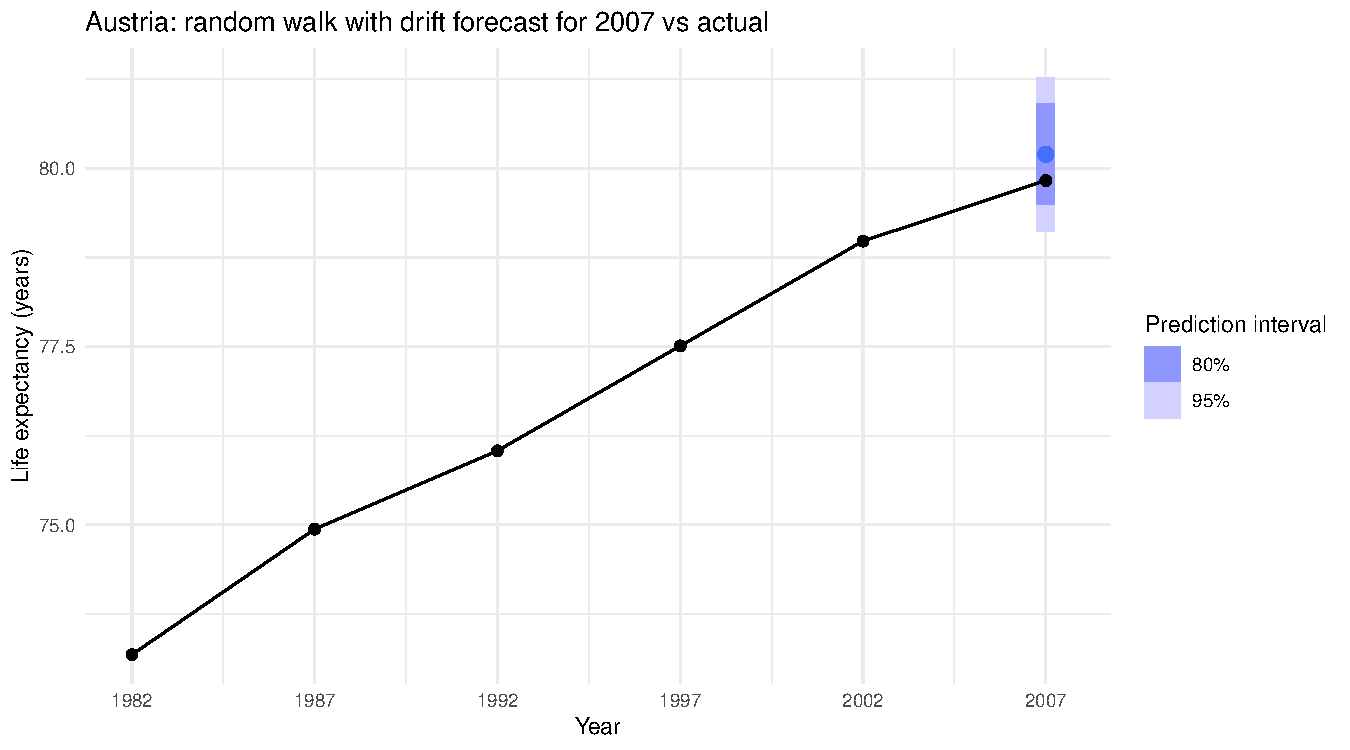
\includegraphics[width=0.9\textwidth]{figures/forecast_Austria_2007.pdf}
    \caption[Forecast of Austria's life expectancy in 2007]{Austria: observed life expectancy (1982--2007 shown) and the random walk with drift forecast for 2007 with its 80\% and 95\% prediction intervals. The black point in 2007 is the actual value.}
    \label{fig:forecast}
\end{figure}

% =====================================================================
\section{Conclusion}
\label{sec:conclusion}

Across countries, life expectancy is strongly associated with income per person and geography. In 1997, a 1\% higher GDP per capita is associated with about 0.056 more years of life expectancy, and African countries lag other continents by 8--9 years even at the same income. Total GDP is a poor substitute for GDP per capita, both in sample and when predicting the 2002 values; a random forest improves the predictions only slightly. Over time, life expectancy in a rich country such as Austria rises so smoothly that a simple trend method forecasts it within a fraction of a year.

\let\enquote\relax
\bibliography{references}

\end{document}